\scanpage{42}
\figure{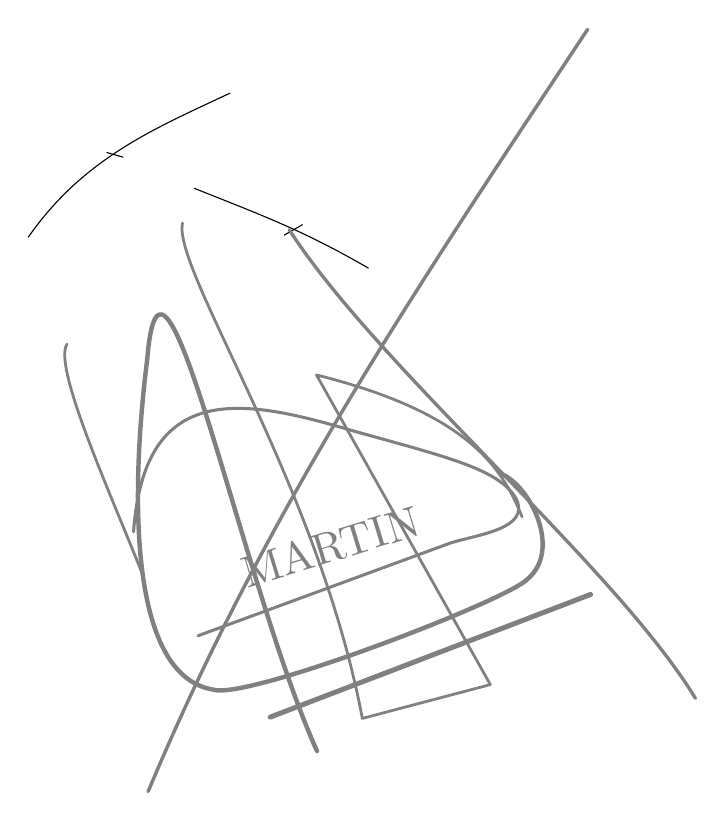
\begin{tikzpicture}[x=.64cm,y=-.53cm,line cap=round,line join=round]
\draw (1.8,6) .. controls (2.9,4.1) and (4.3,3.4) .. (5.8,2.55);
\draw (3.36,3.97)--(3.68,4.08);
\draw (5.1,4.83).. controls (6.6,5.55) and (7.3,5.87)..(8.55,6.74);
\draw (6.88,5.95)--(7.24,5.7);
\draw[gray,line width=1.25pt] (12.9,1.02).. controls (9.4,7.4) and (6.5,12.6)..(4.18,19.28);
\draw[gray,line width=1pt] (4.86,5.66).. controls (4.67,6.8) and (7.55,11.9)..(8.43,17.53)--(10.97,16.72)--(7.52,9.3).. controls (10.5,10.2) and (11.2,11.5)..(11.6,12.7);
\draw[gray,line width=1.2pt] (6.98,5.82).. controls (8.72,9.1) and (13.46,13.9)..(15.04,17.05);
\draw[gray,line width=1.6pt] (7.53,18.31) .. controls (6.03,14.3) and (4.45,4.6) .. (4.16,8.94) .. controls (3.85,11.9) and (3.74,16.5) .. (5.47,16.84) .. controls (6.13,17.1) and (11.27,14.72) .. (11.7,14.2) .. controls (12.4,13.5) and (11.77,11.95) .. (11.17,11.66);
\draw[gray,line width=1pt] (2.57,8.56).. controls (2.27,9.1) and (3.52,12.37)..(4.08,14.12);
\draw[gray,line width=1.1pt] (3.89,13.06).. controls (4.1,9.49) and (5.98,9.83)..(8.16,10.61).. controls (10.04,11.25) and (11.14,11.54)..(11.48,12.26).. controls (11.78,12.99) and (10.72,13.12)..(10.17,13.33)--(5.17,15.55);
\draw[gray,line width=1.8pt] (6.6,17.5)--(12.96,14.56);
\node[rotate=17,scale=1.6,text=gray] at (7.8,13.42){\unsure{MARTIN}};
\end{tikzpicture}}
% crop-candidate: scan 42

\deleted{$A$ anneau noethérien}

\deleted{$x,y\in A$}

\deleted{a) $A/x$, \inserted{$A/y$} réguliers \inserted{intègres} de dim $1$}

\deleted{b) $A$ \inserted{séparé et} complet pour la topologie définie par $xy$}

\diagram{\begin{tikzcd}[ampersand replacement=\&]
\widehat A^{(x)} \& \& {\deleted{\widehat A^{(y)}}}\\
\& A \arrow[ul]\arrow[ur] \&
\end{tikzcd}}

\diagram{\begin{tikzcd}[ampersand replacement=\&]
\widehat X^x \arrow[dr] \& \& {\deleted{\widehat X^y}} \arrow[dl]\\
\& {\deleted{X}} \&
\end{tikzcd}}

\[
\widehat A^{(x,y)}=k[[x,y]]
\]

\figure{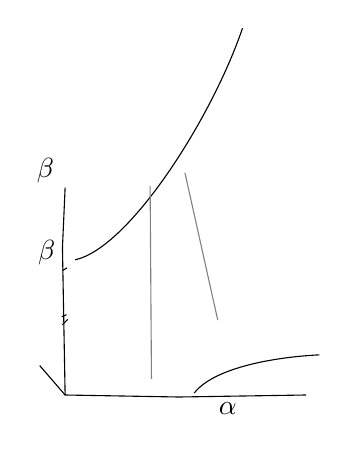
\begin{tikzpicture}[x=.85cm,y=.85cm]
\draw (0,3.1)--(-.04,2.2)--(0,0)--(1.7,-.03)--(3.6,0);
\draw (-.04,1.05)--(.04,1.13) (-.05,1.17)--(.02,1.2) (-.04,1.86)--(.03,1.9);
\node[left] at (-.02,3.35){$\beta$}; \node[left] at (0,2.13){$\beta$}; \node[below] at (2.43,.04){$\alpha$};
\draw (.15,2.02)..controls (.96,2.2) and (2.19,4.13)..(2.65,5.48);
\draw (1.93,.03)..controls (2.2,.38) and (3.02,.56)..(3.8,.6);
\draw[gray,thin] (1.27,3.12)--(1.29,.24) (1.79,3.32)--(2.28,1.12);
\draw (-.38,.44)--(0,0);
\end{tikzpicture}}

\[
\begin{aligned}
\widehat A^{x}&=\left\{\sum a_{\alpha\beta}\,x^{\unsure{\alpha|\gamma}}y^\beta\right\}\\
&\text{\unsure{seul|dont} un nb fini de termes, pour $\alpha\leq N$ donné, sont non nuls}\\
&=k[y][[x]]
\end{aligned}
\]

\[
\begin{aligned}
\widehat A^y&=\left\{\sum a_{\alpha\beta}\,x^\alpha y^\beta\right\}\\
&\text{\unsure{seul|dont} \uline{un} nb fini de termes pour $\beta\leq N$ donné sont non nuls}\\
&=k[x][[y]]
\end{aligned}
\]

\[
\begin{aligned}
&\deleted{\unsure{\beta=}}\\
A&=\left\{\sum a_{\alpha\beta}\,x^\alpha y^\beta\right\}\\
&\text{seul un nb fini des $a_{\alpha\beta}$ pour $\alpha+\beta\leq{}$\uline{$N$ donné}, sont non nuls}
\end{aligned}
\]
% archive sheet number: 41
